%  DOCUMENT CLASS
\documentclass[a4paper,12pt,twoside]{scrreprt}

%PACKAGES
\usepackage[latin1]{inputenc}  % Quelltext ist ISO-8859-1 codiert
\usepackage[ngerman]{babel}
\usepackage[reqno,fleqn]{amsmath}
\setlength\mathindent{10mm}
\usepackage{amssymb}
\usepackage{amsthm}
\usepackage{amsfonts}
\usepackage{extarrows}
\usepackage{fancyhdr}
\usepackage{units}
\usepackage{eurosym}
\usepackage{syntax}
\usepackage{graphicx}

% FORMATIERUNG
\usepackage[paper=a4paper,left=30mm,right=25mm,top=30mm,bottom=35mm]{geometry}
\setlength{\parindent}{0cm}
\setlength{\parskip}{1.5mm plus1mm minus1.5mm}
\addtokomafont{sectioning}{\rmfamily}

%-zusaetzliche Kommandos und Abkuerungen aus externer Datei
\newcommand*{\NN}{\mathbb N}  %Natuerliche Zahlen
\newcommand*{\RR}{\mathbb R}  %Reelle Zahlen
\newcommand*{\CC}{\mathbb C}  %Komplexe Zahlen


\begin{document}
% Seitennummerierung f�r Titel, Widmung, Danksagung, Zusammenfassung
% und Inhaltsverzeichnis werden in roemischen Zahlen gesetzt
\renewcommand{\thepage}{\roman{page}} % Roman page numbers

% Titelblatt
\begin{titlepage}

\title{
  \vspace{2cm}
  \Large{\textbf{
    Universit�t Hamburg\\
    Physikalisches Praktikum f�r Fortgeschrittene\\
    Sommer-Semester 2014
  }}\\
  \vspace{6cm}
  \huge{\textbf{
    Versuch: SALOME (Simple Accelerator for Learning Optics
	and Manipulation of Electrons)
  }}
}

\author{
  \large
  \vspace{4cm}
  \begin{tabular}{ll}
  Praktikanten:&Alexander Okupnik\\
  &Vincent Koppen\\
  Betreuer:\quad&Dr. Velizar Miltchev\\
  \end{tabular}
}

\date{ \large{
    durchgef�hrt vom 1.9. bis zum 5.9.2014
  }}

\end{titlepage}
\maketitle

% Inhalts-, Abbildungs*-, Tabellen*-Verzeichnis
\tableofcontents
\newpage

\renewcommand{\thepage}{\arabic{page}} % Arabic page numbers
\setcounter{page}{1}

% Kapitel
\chapter{Einleitung}

Ziel eines Teilchenbeschleuniger ist es einen Teilchenstrahl oder -bunch zu beschleunigen und m�glichst 
fokussiert auf einer Sollbahn zu halten. Einerseits um keine Teilchen zu verilieren, andersetits um z.B.
bei einem Collider die Teilchendichte hoch zu halten.
In unserem Versuch werden wir mit einem einfachen Linearbeschleuniger arbeiten und die Energie sowie die Emittanz,
eine die Qualit�t des Strahls charakterisierende Gr��e die wir im Theorieteil erkl�ren werden, zu messen.

\section{Aufbau}
\begin{figure}[ht]
  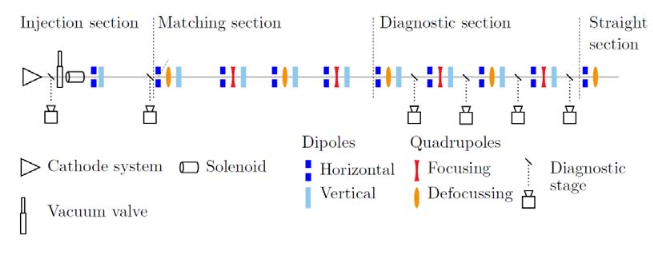
\includegraphics[width=0.8\textwidth]{./salome-aufbau.png}
  \caption{( Matching section wurde abgebaut)}
\end{figure}

Der Teilchenbeschleuniger besteht aus einem Kathodenstrahler zur Erzeugung des Strahls, einer Spule 
(Solenoidmagnet) dessen �u�ere Streufelder fokussierend wirken, einigen Dipol- und Quadromagneten.

\begin{figure}[]
  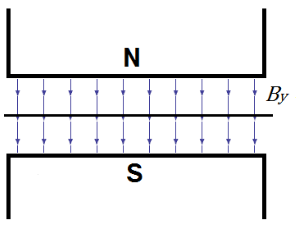
\includegraphics[width=0.40\textwidth]{./dipol.png}\hfill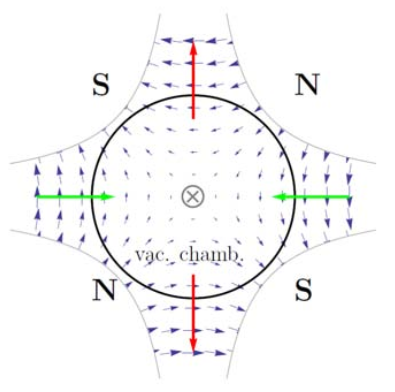
\includegraphics[width=0.40\textwidth]{./quadropol.png}
  \caption{Di-und Quadropolschemata}
  
\end{figure}
\newpage
Wie man im Bild xx illustriert sehen kann erzeugt der Dipolmagnet ein homogenes Magnetfeld in (vertikale) y-Richtung,
das daf�r geeignet ist externe Magnetfelder wie das Erdmagnetfeld zu kompensieren. 
Nehmen wir ein idealisierten Teilchenstrahl an, so lenkt  der Dipol den Strahl auf 
eine Kreisbahn e/p *By= 1/R.

P:Impuls in Richtung der Sollbahn

R:Raidus der Kreisbahn

Die St�rke des Dipols werden wir im Folgendem damit charakterisieren.
Der Quadropol h�ngt linear von x ab und wirkt in einer ebene fokussierend in der anderen defokussierend, 
deswegen werden sie um 90� gedreht hintereinander aufgebaut.

e/p*By(x)=kx

e/p*Bx(y)=-ky

k: St�rke des Quadropolmagneten

\newpage
\section{Theorie}
\section {Phasenraum, Emittanz und Twissparameter}
Man stellt zun�chst die Bewegungsgleichungen eines einzelnen Teilchens auf und guckt wie dieses sich unabh�ngig 
von den anderen Teilchen im Bezug auf die Sollbahn bewegt. Den Einfluss der Teilchen aufeinander kann hier 
vernachl�ssigt werden da der Strom sehr klein ist und vorrausgesetzt wird, dass sich die Sollbahn nicht gekr�mmt ist.

\begin{equation}x''(s)-k(s)x(s)=0
\end{equation}

\begin{equation}y''(s)+k(s)y(s)=0
\end{equation}

s parametrisiert die Sollbahn.

Die Herleitung der Differentialgleichung findet man im Wille S. xx.  

Hier sieht man das die Bewegung in x und y Richtung entkoppelt ist und die

Fokussierung/Defokussierung in beiden Ebenen gerade umgekehrt ist.

Die L�sung der Gleichung ist analytisch schwierig, da sich k entlang der Bahn s �ndert, jedoch kann man jeden Abschnitt in der Sollbahn wo sich
k �ndert f�r sich betrachten und so ein Kalk�l entwickeln der die Bewegungsgleichung in diskreten Abschnitten mithilfe von Matrizen l�st.
M�chte man zb. f�r gegebene Anfangswerte x0 und x'0 des Teilchens die Werte x1, x'1 ermitteln nachdem es einen Dipol und Quadropol durchlaufen hat,
so nimmt man die einzelnen Matrizen f�r Dipol und Quadropol und f�hrt sie hintereinander aus.

Diesen Kalk�l werden wir sp�ter in der Berechnung der Emittanz verwenden.

Das Teilchen f�hrt eine oszillierende Bewegung um die Sollbahn durch.Im Phasenraum ist die Bewegung durch eine Ellipse beschrieben:

\begin{equation}
\epsilon=\gamma(s)x^2(s)+2\alpha(s)x(s)x'(s)+\beta(s)x'^2(s)\end{equation}

x(s) ist die Ablenkung zur Sollbahn, x'(s) Der Winkel zwischen Geschwindigkeit und Sollbahn. 

$\gamma(s),\alpha(s),\beta(s)$ sind die sogenannten ``Twissparameter'', sie bestimmen die Form und Position der Ellipse, und sind
auch abh�ngig von der Position auf der Sollbahn. Sie werden allein durch den Aufbau bzw. der Fokussierung entlang der Sollbahn 
bestimmt und unabh�ngig von den Anfangsbedingungen.

Die Anfangsbedingungen x0 und x'0 gehen in die Integrationskonstanten $\epsilon$ und der Anfangsphase $\Phi$ der Schwingung ein.

$\epsilon$ ist die sogenannte Emittanz des Teilchens und wurde als Integrationskonstante eingef�hrt. Sie ist daher eine 
Erhaltungsgr��e und nach der Gleichung im Phasenraum auch die Fl�che der Ellipse bis auf einen Faktor $\pi$.
Sie charakterisiert somit die Qualit�t und die Fokussierbarkeit des Strahls.

Im n�chsten Schritt wollen wir charakteristische Gr��en f�r den Teilchenstrahl, bestehend aus mehreren Teilchen die den selben Differentialgleichungen
unterliegen, festlegen. Da die Twissparameter unabh�ngig von den Anfangsbedingungen die Ellipse entlang s verformen, liegen Teilchen mit gleicher Emittanz
an verschiedenen Punkten derselben Ellipse oder sie haben verschiedene Emittanzen und bewegen sich innerhalb einer kleineren bzw. gr��eren Ellipse.

Wir definieren die Emittanz des gesamten Teilchensstrahles als die Fl�che der Ellipse die von der Standardabweichungen von x und x' aufgespannt wird.

Da sich die so definierte Emittanz mit Beschleunigung verkleinert f�hren wir die normierte Emittanz ein :

\begin{equation}
\epsilon_n=\gamma \beta \sqrt{<x^2>*<x'^2>-(<x><x'>)^2}\end{equation}

mit dem Lorentzfaktor $\gamma$ und $\beta=v/c$ 






\chapter{Energiemessung}
\section{}

Zun�chst wollen wir eine sogenannte Energiemessung durchf�hren. Die
Elektronen, aus dem der Strahl des Beschleunigers besteht, werden
am Anfang des Aufbaus thermisch durch die Kathode erzeugt erhalten
somit ihre kinetische Energie und Impuls(-betrag), die sich von da
an nicht ver�ndern.
\chapter{Emittanzmessung}

An jedem Punkt $z$ entlang des Orbits hat der Elektronenstrahl
unter Anderem die Gr��en $\langle x^2\rangle(z)$, $\langle xx'\rangle(z)$,
$\langle x'^2\rangle(z)$, bzw.
$\langle y^2\rangle(z)$, $\langle yy'\rangle(z)$, $\langle y'^2\rangle(z)$. Wenn
$R = \bigl(\begin{smallmatrix} R_{11}&R_{12}\\ R_{21}&R_{22}
\end{smallmatrix} \bigr)$ die Transformationsmatrix der Gr��en $x$
und $x'$ eines einzelnen Elektrons von $z_0$ zu $z_1$ ist,
dann gilt
\begin{equation}
	\langle x^2\rangle(z_1) =
	\begin{pmatrix} R_{11}^2 & 2R_{12}R_{11} & R_{12}^2 \end{pmatrix}
	\begin{pmatrix} \langle x^2\rangle(z_0)\\\langle xx'\rangle(z_0)
					\\\langle x'^2\rangle(z_0) \end{pmatrix} \text{,}
\end{equation}
und es gilt Analoges f�r $y$.

F�r die entlang des Orbits erhaltene Emittanz $\eps$ gilt
\begin{equation}
		\eps = \sqrt{\langle x^2\rangle(z)\langle x'^2\rangle(z)
		- \langle xx'\rangle(z)^2} \quad \forall z
\end{equation}

Wir werden hierzu die Gr��en $a_1 := \langle x^2\rangle$, $a_2 := \langle
xx'\rangle$ und
$a_3 := \langle x'^2\rangle$ (und alles Folgende analog f�r $y$) direkt vor dem
Quadrupolmagneten
V46MATCH bestimmen und daraus dann die transversalen Emittanzen $\eps_x$ und
$\eps_y$ und ihre normierten Varianten $\eps_{x,n}$ und $\eps_{y,n}$ erhalten.

F�r ersteres werden wir den Elektronenstrahl $n$-mal auf verschiedene Weise
transformieren (�ber verschiedene Strecken oder Optiken), wobei $b_i$
die Gr��e $\langle x^2\rangle$ nach der $i$-ten Transformation und
$R^{(i)}$ die entsprechende Transformationsmatrix ist.
Das f�r gro�es $n$ �berbestimmte lineare Gleichungssystem
\begin{equation}
 \begin{pmatrix} b_1 \\ \vdots \\ b_n \end{pmatrix} = \underbrace{
 \begin{pmatrix} {R^{(1)}_{11}}^2 & 2R^{(1)}_{12}R^{(1)}_{11} & {R^{(1)}_{12}}^2 \\
				 & \vdots & \\
				 {R^{(n)}_{11}}^2 & 2R^{(n)}_{12}R^{(n)}_{11} & {R^{(n)}_{12}}^2 \\
 \end{pmatrix} }_{=:B}
 \begin{pmatrix} a_1 \\ a_2 \\ a_3 \end{pmatrix}
\end{equation}
an die zu ermitteltenden Unbekannten $a_1$, $a_2$, $a_3$ kann und wird dann
Grundlage f�r einen $\chi^2$-Fit sein.

\section{Messung durch Variation des Quadrupolstroms}

Zuerst lassen wir den Elektronenstrahl von dem Punkt direkt vor
V46MATCH bis zum Schirm 2 auf verschiedene Weise transformieren, indem
wir an V46MATCH jeweils 25, bzw. 19 verschiedene Stromst�rken einstellen und dann
$\langle x^2 \rangle$, bzw. $\langle y^2 \rangle$ an Schirm 3 messen. Die
Messergebnisse sind in den Tabellen \ref{tab:xemitquad} und \ref{tab:yemitquad}
dargestellt.

\begin{table}[ht]
\centering
\begin{tabular}{| >{$}c<{$} >{$}c<{$} |}
\hline
I\text{ [A]}	&	\langle x^2 \rangle \text{ [mm]}	 \\ [0.2ex]
\hline\hline
0,70	&	0,66	\\
0,75	&	0,616	\\
0,80	&	0,58	\\
0,85	&	0,55	\\
0,90	&	0,5	\\
0,95	&	0,48	\\
1,00	&	0,44	\\
1,05	&	0,4	\\
1,10	&	0,4	\\
1,15	&	0,39107	\\
1,20	&	0,382277	\\
1,25	&	0,381375	\\
1,30	&	0,380214	\\
1,35	&	0,396236	\\
1,40	&	0,403774	\\
1,45	&	0,429807	\\
1,50	&	0,450623	\\
1,55	&	0,466817	\\
1,60	&	0,500828	\\
1,65	&	0,525564	\\
1,70	&	0,548818	\\
1,75	&	0,572263	\\
1,80	&	0,627355	\\
1,85	&	0,659232	\\
1,90	&	0,673288	\\

\hline
\end{tabular}
\caption{Messung der horizontalen Strahlgr��e $\langle x^2 \rangle$ an Schirm 2
			in Abh�ngigkeit des Quadrupolstroms $I$ bei V46MATCH.}
	\label{tab:xemitquad}
\end{table}

\begin{table}[ht]
\centering
\begin{tabular}{| >{$}c<{$} >{$}c<{$} |}
\hline
I\text{ [A]}	&	\langle y^2 \rangle \text{ [mm]}	 \\ [0.2ex]
\hline\hline


\hline
\end{tabular}
\caption{Messung der vertikalen Strahlgr��e $\langle y^2 \rangle$ an Schirm 2
			in Abh�ngigkeit des Quadrupolstroms $I$ bei V46MATCH.}
	\label{tab:yemitquad}
\end{table}




\section{Messung durch Variation der Schirme}
\chapter{Strahlf�hrung}

\section{\emph{Beam-based Alignment}}

Wenn der Elektronenstrahl nicht mittig durch einen Quadrupolmagneten f�hrt,
dann wirkt dieser nicht nur (de-)fokussierend, sondern auch den ganzen Strahl
ablenkend. Daher liegt der Wunsch nahe, dass der Elektronenstrahl von den
Dipolmagneten so gelenkt wird, dass er mittig durch die Quadrupole l�uft.
Wir werden im Folgenden solche Stromwerte f�r den horizontalen Dipol Q1MATCH und
den vertikalen Dipol H15MATCH finden, dass der Strahl mittig durch den
Quadrupolmagneten V46MATCH f�hrt.

Dies geschieht, indem wir jeweils f�r zwei verschiedene Quadrupolstr�me die
(lineare) Abh�ngigkeit des Versatzes des Strahls auf Schirm 3 von dem
Dipolstrom messen. Der Schnittpunkt der Geraden, die diese linearen Abh�ngigkeiten
beschreiben, entspricht dann dem Dipolstrom, bei dem der Versatz des
Elektronenstrahls bei zwei verschiedenen Quadrupolstr�men auf Schirm 3 gleich ist,
der Quadrupol also zu keiner Ablenkung f�hrt. D.h. bei dem gefundenen Dipolstrom
l�uft der Strahl mittig durch den Quadrupolmagneten.

Die Messung verlief analog zu vorherigen Messungen der Strahlpositionen auf
einem Schirm mithilfe des Bildanalyse-Programms. Die Messergebnisse sind
in den Tabellen \ref{tab:xbeamalign} und \ref{tab:ybeamalign} sowie 
graphisch in den Abbildungen \ref{fig:xbeamalign} und
\ref{fig:ybeamalign} dargestellt. Dort sind auch die jeweiligen
berechneten Regressionsgeraden eingezeichnet.

F�r die horizontale Richtung $x$ erhalten wir als Schnittpunkt der beiden
(2A)- und (1A)-Regressionsgeraden (siehe Bildunterschrift zu Abbildung
\ref{fig:xbeamalign}) einen Stromwert von $I_\text{Q1MATCH} = -3,055 \text{ A}$.

Diesen stellen wir am Dipol Q1MATCH ein und variieren den Quadrupolstrom,
um zu verifizieren, dass wir einen Dipolstrom $I_\text{Q1MATCH}$ gefunden haben,
bei dem der Quadrupol keinen Einfluss auf die $x$-Ablenkung des Strahls �berhalb
der Messungenaugkeit hat. Man sieht in Tabelle \ref{tab:xbeamaligncheck},
dass dies der Fall ist.

F�r die vertikale Richtung $y$ erhalten wir als Schnittpunkt der beiden
(0A)- und (1A)-Regressionsgeraden (siehe Bildunterschrift zu Abbildung
\ref{fig:ybeamalign}) einen Stromwert von $I_\text{H15MATCH} = 2,211 \text{ A}$.

Auch dieser ist, wovon wir uns vergewissert haben, derart, dass der
Elektronenstrahl nun bei Variation des Quadrupolstromes einen im
Rahmen der Messungenauigkeit von 0,25 mm konstanten $y$-Versatz auf
Schirm 3 hat.

\begin{table}[ht]
\centering
\begin{tabular}{| >{$}c<{$} | >{$}c<{$} >{$}c<{$} |}
\hline
& I_\text{V46MATCH}=2{ A} & I_\text{V46MATCH}=1{ A}		 \\ [0.2ex]
\hline
\hline
I_\text{Q1MATCH}{ [A]}	&	\langle x \rangle \text{ [mm]}
							&	\langle x \rangle \text{ [mm]}	 \\ [0.2ex]
\hline\hline
-3,2	&	4,211931	&	4,635957	\\
-3,1	&	3,561591	&	3,668923	\\
-3,0	&	2,796788	&	2,647021	\\
-2,9	&	2,083065	&	1,60043		\\
-2,8	&	1,353469	&	0,577545	\\
-2,7	&	0,658561	&	-0,444051	\\
-2,6	&	-0,019461	&	-1,53573	\\
-2,5	&	-0,836498	&	-2,562317	\\
-2,4	&	-1,574353	&	-3,671382	\\
-2,3	&	-2,372214	&	-4,725614	\\
-2,2	&	-3,133507	&	-5,859231	\\
-2,1	&	-3,916701	&	-6,973545	\\
-2,0	&	-4,636089	&	-8,073133	\\
\hline
\end{tabular}
\caption{Messung des $x$-Versatzes des Strahls auf Schirm 3 in Abh�ngigkeit
 			des Stroms $I_\text{Q1MATCH}$ des horizontalen Dipols bei zwei
			verschiedenen Quadrupolstr�men $I_\text{V46MATCH}$.}
 	\label{tab:xbeamalign}
\end{table}

\begin{table}[ht]
\centering
\begin{tabular}{| >{$}c<{$} | >{$}c<{$} >{$}c<{$} |}
\hline
& I_\text{V46MATCH}=0{ A} & I_\text{V46MATCH}=1{ A}		 \\ [0.2ex]
\hline
\hline
I_\text{H15MATCH}{ [A]}	&	\langle y \rangle \text{ [mm]}
							&	\langle y \rangle \text{ [mm]}	 \\ [0.2ex]
\hline\hline
1,4	&	-11,12211	&	-5,888465	\\
1,5	&	-9,723441	&	-5,182737	\\
1,6	&	-7,899436	&	-4,522313	\\
1,7	&	-6,663419	&	-3,781678	\\
1,8	&	-5,849714	&	-3,102607	\\
1,9	&	-4,314929	&	-2,454651	\\
2,0	&	-3,065036	&	-1,702393	\\
2,1	&	-1,413789	&	-1,053516	\\
2,2	&	-0,588087	&	-0,342917	\\
2,3	&	0,985734	&	0,509527	\\
2,4	&	1,463655	&	1,18625		\\
\hline
\end{tabular}
\caption{Messung des $y$-Versatzes des Strahls auf Schirm 3 in Abh�ngigkeit
 			des Stroms $I_\text{H15MATCH}$ des vertikalen Dipols bei zwei
			verschiedenen Quadrupolstr�men $I_\text{V46MATCH}$.}
 	\label{tab:ybeamalign}
\end{table}

\begin{figure}[ht]
    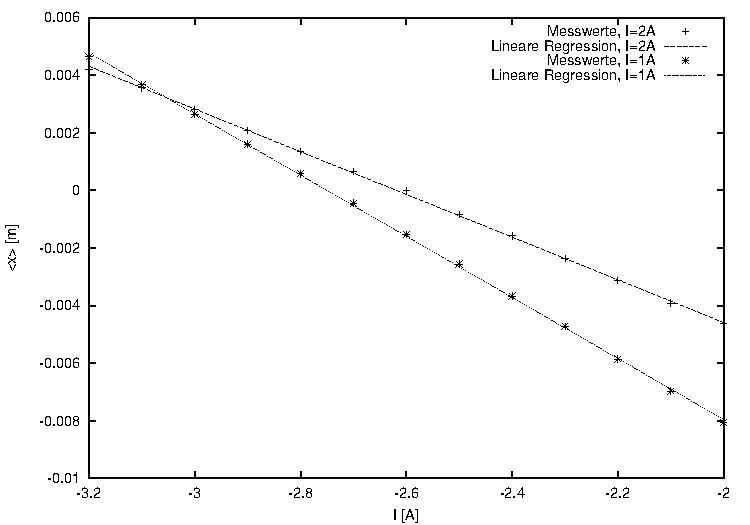
\includegraphics[width=1\textwidth]{./xbeamalignment.pdf}
	\caption{Messung des $x$-Versatzes des Strahls auf Schirm 3 in Abh�ngigkeit
 			des Stroms $I_\text{Q1MATCH}$ des horizontalen Dipols bei zwei
			verschiedenen Quadrupolstr�men $I_\text{V46MATCH}$
			(vgl. Tabelle \ref{tab:xbeamalign}).
			(2A)-Regressionsgerade gegeben durch
			$\frac{\langle x\rangle}{m}
				= -0,00741\cdot \frac{I}{\text{A}} - 0,01941$,
			(1A)-Regressionsgerade gegeben durch
			$\frac{\langle x\rangle}{m} 
				= -0,01061\cdot \frac{I}{\text{A}} - 0,02918$.}
			\label{fig:xbeamalign}
\end{figure}

\begin{figure}[ht]
    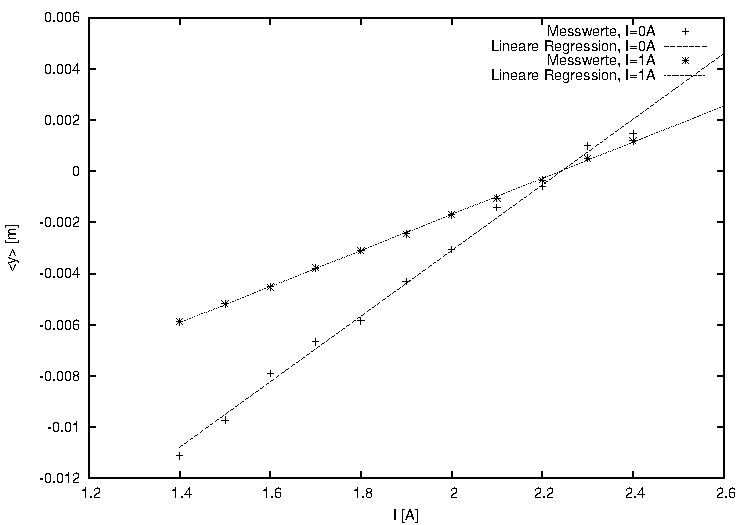
\includegraphics[width=1\textwidth]{./ybeamalignment.pdf}
	\caption{Messung des $y$-Versatzes des Strahls auf Schirm 3 in Abh�ngigkeit
 			des Stroms $I_\text{H15MATCH}$ des vertikalen Dipols bei zwei
			verschiedenen Quadrupolstr�men $I_\text{V46MATCH}$
			(vgl. Tabelle \ref{tab:ybeamalign}).
			(0A)-Regressionsgerade gegeben durch
			$\frac{\langle y\rangle}{m}
				= 0,0128 \cdot \frac{I}{\text{A}} - 0,0287$,
			(1A)-Regressionsgerade gegeben durch
			$\frac{\langle y\rangle}{m}
				 = 0,00704 \cdot \frac{I}{\text{A}} - 0,01579$.}
			\label{fig:ybeamalign}
\end{figure}

\begin{table}[ht]
\centering
\begin{tabular}{| >{$}c<{$} >{$}c<{$} |}
\hline
I_\text{V46MATCH}{ [A]}	&	\langle x \rangle \text{ [mm]}	 \\ [0.2ex]
\hline\hline
1,0	&	3,232253	\\
0,8	&	3,183226	\\
0,6	&	3,175869	\\
0,4	&	3,127449	\\
0,2	&	3,165518	\\
0,0	&	3,147471	\\
\hline
\end{tabular}
\caption{$x$-Versatz auf Schirm 3 f�r verschiedene Quadrupolstr�me bei
			$I_\text{Q1MATCH} = -3,055 \text{ A}$.}
	\label{tab:xbeamaligncheck}
\end{table}
\chapter{Fehlerdiskussion}
\section{Energiemessung}

In unserer ersten Messung bestimmen wir die kinetische Energie der Elektronen mithilfe 
des linearen Zusammenhanges zwischen Ablenkung des Strahls im homogenen Magnetfeld
und der Magnetfeldst�rke.
Jede Messung hatte eine Messungenauigkeit von 0,25 mm durch die Pixelgr��e der Kamera,
die wir zur Aufnahme der Strahlposition verwendet haben. Da diese Ungenauigkeit bei jedem Messpunkt 
gleich war, haben wir bei der linearen Regression keine Gewichtung der einzelnen Messpunkte vorgenommen.

Das Messergebnis war : $E_\text{kin}$ = (7,2 $\pm$ 0,2) keV

Eine Ursache der Ungenauigkeit bei der Messung k�nnte die statistische Verteilung der 
kinetischen Energien der Teilchen durch die thermische Erzeugung in der Kathode sein.
Teilchen mit verschiedenen Energien w�rden auch anders im Magnetfeld abgelenkt,
jedoch w�rde das in erster Linie zu einer Verbreiterung des Strahles in 
$y$-Richtung f�hren, was wir mit blo�em Auge nicht beobachten konnten.
Nichtsdestotrotz k�nnte man zur Verbesserung der Messung eine genauere
Elektronenstrahlquelle verwenden.


\section{Erste und zweite Emittanzmessung}

Die Emittanz hatten wir auf zwei verschiedene Arten gemessen.
Einmal durch Messung der Strahlgr��e bei Variation des Quadropolstromes an einem Schirm 
und einmal die Messung bei gleichem Quadrupolstrom an vier verschiedenen Schirmen.
Wir haben, wie ihn Kapitel 3 beschrieben, zur Bestimmung der Gr��en $\langle x^2 \rangle$,
$\langle xx' \rangle$ und $\langle x'^2 \rangle$ einen $\chi^2$-Fit durchgef�hrt, und
aus diesen drei Gr��en die Emittanz mit Fehlerfortpflanzung errechnet.

Dabei f�llt nat�rlich auf, dass eine Messung mit drei Freiheitsgraden und nur vier Messpunkten wie es
bei der Schirmvariationsmessung der Fall ist, eine statistische Fehleranalyse mit einem $\chi^2$-Fit wenig Aussagekraft hat.

Messung 1: \begin{equation}\eps_{x,n} = (0,136 \pm 0,005)\text{ mm}\cdot\text{mrad.} \nonumber \end{equation}
            \begin{equation}\eps_{y,n} = (0,222 \pm 0,011)\text{ mm}\cdot\text{mrad.} \nonumber\end{equation}

Messung 2: \begin{equation}\eps_{x,n} = (0,119 \pm 0,016)\text{ mm}\cdot\text{mrad} \nonumber \end{equation}
            \begin{equation}\eps_{y,n} = (0,35 \pm 0,02)\text{ mm}\cdot\text{mrad.} \nonumber\end{equation}           

In unseren Rechnungen haben wir �u�ere St�rfelder zb. durch die Messger�te nicht beachtet, obwohl sie gro�en Einfluss auf die Bahn haben k�nnen. Ein Hinweis darauf sind schon die 
hohen Stromwerte an den Dipolmagneten, die allein bei der Strahlf�hrung verwendet werden m�ssen.

In den theoretischen Vorhersagen wurden �u�ere Multipol-St�rfelder,
die im Strahlrohr vorhanden sind, nicht ber�cksichtigt. Au�erdem f�hren
Hysterese-Effekte der Magneten f�r eine Diskrepanz zwischen theoretischem
Magnetfeld und tats�chlichem.

Die leichte Beeinflussung des Elektronenstrahles durch �u�ere St�rfelder kann man auch sehen, wenn man ein Handy an den Kathodenstrahler h�lt und auf dem n�chsten Schirm sieht 
wie stark sich dann die mittlere Position des Strahles �ndert.

Weiter hatten wir angenommen, dass die Bewegung des Strahles in den Komponenten x und y entkoppelt sind. Dies ist eine grobe N�herung, die nicht der Realit�t entspricht.

Die statistischen Fehler durch die Fehlerfortpflanzung h�ngen auch von den Matrizen ab, die wir zb. in Gleichung \eqref{emittanz} verwendet haben. Verschiedene Stromwerte 
f�r die Quadropole �ndern die Matrixeintr�ge und somit die Gr��e der Fehler.

Eine Idee zur Eind�mmung dieses Problemes w�re die Messung mit verschiedenen Quadropol-Einstellungen durchzuf�hren und gucken bei welchem die Standardabweichung der  
Emittanz sinkt. 

\section{Beam-based Alignment}

In dem ``Beam-based Alignment'' haben wir an einem Schirm die Strahlposition bei variierender Dipolablenkung gemessen. 

F�r zwei verschiedene Quadropolstr�me haben wir die Messwerte aufgetragen und geguckt, wo sich die Geraden schneiden.

$x$-Dipol (Q1Match) $I$ = -3.055A

$y$-Dipol (H15Match) $I$ = 2.211A

Um die Werte zu testen, haben wir die Dipole auf diese Werte eingestellt und den Quadropol von -2A bis 2A laufen lassen und geguckt, ob sich die Strahlmitte verschiebt.

Die Verschiebung fand im Rahmen der Messungenauigkeit statt, sodass wir davon ausgehen k�nnen, dass wir sehr gute Werte erreicht haben.


\chapter{}
\section{}

% Literaturverzeichnis mit File literatur.tex
\chapter{Literaturverzeichnis}
[1]	 V.Wacker Versuchsmappe SALOME
        
         http://www.physik.uni-hamburg.de/ex/html/fprakt/e/Beschleuniger/SALOME_VersMappe_a.pdf

[2]      K. Wille. \emph{Physik der Teilchenbeschleuniger und Synchrotonstrahlungsquellen}. Teubner Studienb�cher, 1996.



\end{document}

